\begin{problem}{셔틀버스}{standard input}{standard output}

서울대학교 내부를 운행하는 셔틀버스에는 한쪽 벽면에 $N$개의 좌석이 일렬로 놓여 있다. 각 좌석은 가장 왼쪽 좌석부터 시작하여 1번부터 $N$번까지의 번호가 붙어 있다. 이 버스는 학교 입구에서 $N$명의 학생들을 태운 뒤 출발하고, 학생들은 각자 하나의 좌석을 골라 앉는다. 편의상 출발할 때 $i$번 좌석에 앉은 학생을 $i$번 학생으로 부르기로 한다.

\begin{center}
  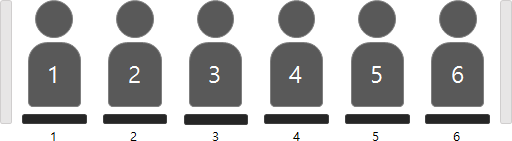
\includegraphics[width=0.5\textwidth]{bus1.png}
\end{center}
학생들은 칸막이에 기대서 조는 것을 좋아하기 때문에 되도록 양쪽 끝자리에 앉고 싶어 한다. 그래서 바로 옆에 앉아 있던 학생이 내리거나 다른 자리로 옮겨 가서 좌석이 비었을 때 그 좌석으로 옮겨 앉는 게 양쪽 끝 자리에 더 가까워질 경우, 즉 $1$번 좌석과 $N$번 좌석 중 더 가까운 좌석까지의 거리가 줄어들 경우 그 좌석으로 옮겨 앉는다. 한 학생이 버스에서 내리는 즉시 모든 학생이 이 규칙에 따라 이동한다.

셔틀버스 기사 찬수는 버스에서 내리는 학생들을 보면서 지금 어떤 좌석에 어떤 학생이 앉아 있는지 궁금해졌다. 찬수를 위해 아래의 두 가지 연산을 입력되는 순서대로 수행하는 프로그램을 작성해 주자.

\begin{enumerate}
\item{\texttt{1 x} : $x$번 학생이 버스에서 내린다. 이 학생은 버스에 타고 있던 학생임이 보장된다.}
\item{\texttt{2 x} : $x$번 좌석에 앉아 있는 학생의 번호를 출력한다. 좌석이 비어 있을 경우는 \texttt{0}을 출력한다.}
\end{enumerate}

찬수가 운전하는 버스는 차고지로 들어가는 버스이기 때문에 새로운 학생을 태우지는 않는다.

\InputFile
첫 번째 줄에 셔틀버스에 있는 좌석의 수 $N$($1 \le N \le 100,000$), 처리해야 하는 연산의 수 $M$($1 \le M \le 200,000$)이 주어진다.

두 번째 줄부터 $M$개의 줄에 걸쳐 각 쿼리의 종류(\texttt{1} 또는 \texttt{2})와 $x$($1 \le x \le N$) 값이 공백을 사이에 두고 주어진다. 2번 쿼리가 하나 이상 존재함이 보장된다.

\OutputFile
각 2번 쿼리의 결과를 입력되는 순서대로 한 줄에 하나씩 출력한다.

\Example

\begin{example}
\exmp{6 9
2 2
1 1
2 1
2 6
1 3
2 4
1 5
2 5
2 3}{2
2
6
4
4
0}%
\end{example}

\Notes

\begin{center}
  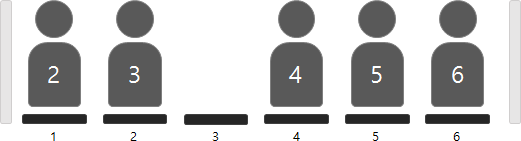
\includegraphics[width=0.5\textwidth]{bus2.png}
\end{center}
1번 학생이 내리면 2번 학생과 3번 학생이 순서대로 이동한다. 4번 학생은 3번 좌석으로 옮겨 앉더라도 양 끝 좌석까지의 거리가 변하지 않기 때문에 이동하지 않는다.

\begin{center}
  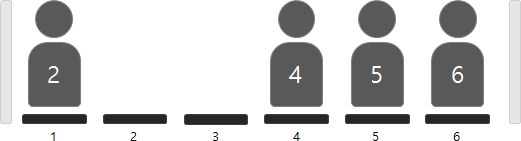
\includegraphics[width=0.5\textwidth]{bus3.png}
\end{center}
3번 학생이 내리면 4번 학생은 2번 좌석으로 이동하는 것이 이득이지만, 바로 옆자리가 아니므로 이동하지 않는다.

\begin{center}
  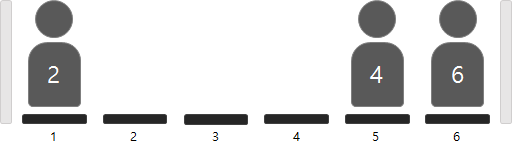
\includegraphics[width=0.5\textwidth]{bus4.png}
\end{center}
5번 학생이 내리면 4번 학생이 이동한다.

\end{problem}
